\documentclass{standalone}
\usepackage{tikz}
\usepackage{hsbcommon}

\begin{document}  

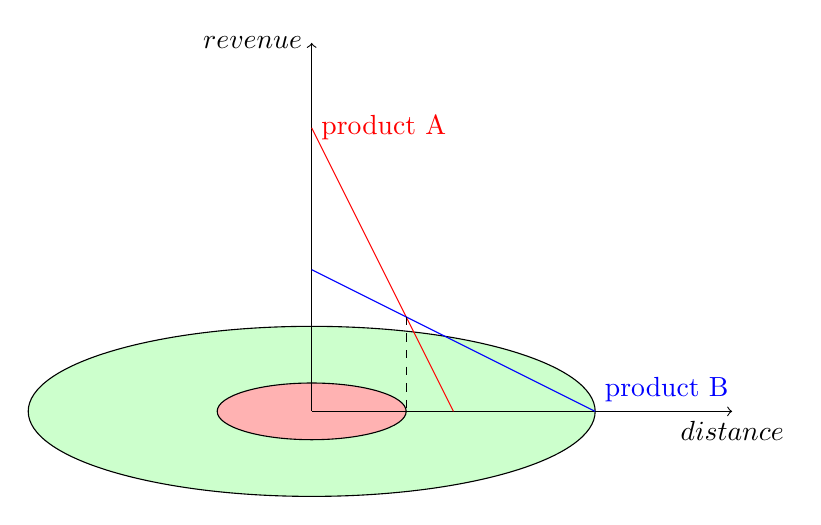
\begin{tikzpicture} [scale=0.6]

    \begin{scope}[yscale=0.3]
        \draw[fill=green!20] (0,0) circle (6);    
        \draw[fill=red!30] (0,0) circle (2);            
    \end{scope}
    
    %Axis
    \draw [<-] (0,7.8) node [left] {$revenue$} -- (0,0);
    \draw[->] (0,0) -- (8.9,0) node [below] {$distance$};

    \draw[red] (0,6) node[right] {product A} -- (3,0);
    \draw[blue] (0,3) -- (6,0) node[above right] {product B};

    \draw[dashed] (2,2) -- (2,0);

    
    
  
\end{tikzpicture}

\end{document}
